\documentclass[]{article}
\usepackage{lmodern}
\usepackage{amssymb,amsmath}
\usepackage{ifxetex,ifluatex}
\usepackage{fixltx2e} % provides \textsubscript
\ifnum 0\ifxetex 1\fi\ifluatex 1\fi=0 % if pdftex
  \usepackage[T1]{fontenc}
  \usepackage[utf8]{inputenc}
\else % if luatex or xelatex
  \ifxetex
    \usepackage{mathspec}
  \else
    \usepackage{fontspec}
  \fi
  \defaultfontfeatures{Ligatures=TeX,Scale=MatchLowercase}
\fi
% use upquote if available, for straight quotes in verbatim environments
\IfFileExists{upquote.sty}{\usepackage{upquote}}{}
% use microtype if available
\IfFileExists{microtype.sty}{%
\usepackage{microtype}
\UseMicrotypeSet[protrusion]{basicmath} % disable protrusion for tt fonts
}{}
\usepackage[margin=1in]{geometry}
\usepackage{hyperref}
\hypersetup{unicode=true,
            pdftitle={Multiplicative input noise infusion},
            pdfauthor={Lars Vilhuber},
            pdfborder={0 0 0},
            breaklinks=true}
\urlstyle{same}  % don't use monospace font for urls
\usepackage{color}
\usepackage{fancyvrb}
\newcommand{\VerbBar}{|}
\newcommand{\VERB}{\Verb[commandchars=\\\{\}]}
\DefineVerbatimEnvironment{Highlighting}{Verbatim}{commandchars=\\\{\}}
% Add ',fontsize=\small' for more characters per line
\usepackage{framed}
\definecolor{shadecolor}{RGB}{248,248,248}
\newenvironment{Shaded}{\begin{snugshade}}{\end{snugshade}}
\newcommand{\KeywordTok}[1]{\textcolor[rgb]{0.13,0.29,0.53}{\textbf{{#1}}}}
\newcommand{\DataTypeTok}[1]{\textcolor[rgb]{0.13,0.29,0.53}{{#1}}}
\newcommand{\DecValTok}[1]{\textcolor[rgb]{0.00,0.00,0.81}{{#1}}}
\newcommand{\BaseNTok}[1]{\textcolor[rgb]{0.00,0.00,0.81}{{#1}}}
\newcommand{\FloatTok}[1]{\textcolor[rgb]{0.00,0.00,0.81}{{#1}}}
\newcommand{\ConstantTok}[1]{\textcolor[rgb]{0.00,0.00,0.00}{{#1}}}
\newcommand{\CharTok}[1]{\textcolor[rgb]{0.31,0.60,0.02}{{#1}}}
\newcommand{\SpecialCharTok}[1]{\textcolor[rgb]{0.00,0.00,0.00}{{#1}}}
\newcommand{\StringTok}[1]{\textcolor[rgb]{0.31,0.60,0.02}{{#1}}}
\newcommand{\VerbatimStringTok}[1]{\textcolor[rgb]{0.31,0.60,0.02}{{#1}}}
\newcommand{\SpecialStringTok}[1]{\textcolor[rgb]{0.31,0.60,0.02}{{#1}}}
\newcommand{\ImportTok}[1]{{#1}}
\newcommand{\CommentTok}[1]{\textcolor[rgb]{0.56,0.35,0.01}{\textit{{#1}}}}
\newcommand{\DocumentationTok}[1]{\textcolor[rgb]{0.56,0.35,0.01}{\textbf{\textit{{#1}}}}}
\newcommand{\AnnotationTok}[1]{\textcolor[rgb]{0.56,0.35,0.01}{\textbf{\textit{{#1}}}}}
\newcommand{\CommentVarTok}[1]{\textcolor[rgb]{0.56,0.35,0.01}{\textbf{\textit{{#1}}}}}
\newcommand{\OtherTok}[1]{\textcolor[rgb]{0.56,0.35,0.01}{{#1}}}
\newcommand{\FunctionTok}[1]{\textcolor[rgb]{0.00,0.00,0.00}{{#1}}}
\newcommand{\VariableTok}[1]{\textcolor[rgb]{0.00,0.00,0.00}{{#1}}}
\newcommand{\ControlFlowTok}[1]{\textcolor[rgb]{0.13,0.29,0.53}{\textbf{{#1}}}}
\newcommand{\OperatorTok}[1]{\textcolor[rgb]{0.81,0.36,0.00}{\textbf{{#1}}}}
\newcommand{\BuiltInTok}[1]{{#1}}
\newcommand{\ExtensionTok}[1]{{#1}}
\newcommand{\PreprocessorTok}[1]{\textcolor[rgb]{0.56,0.35,0.01}{\textit{{#1}}}}
\newcommand{\AttributeTok}[1]{\textcolor[rgb]{0.77,0.63,0.00}{{#1}}}
\newcommand{\RegionMarkerTok}[1]{{#1}}
\newcommand{\InformationTok}[1]{\textcolor[rgb]{0.56,0.35,0.01}{\textbf{\textit{{#1}}}}}
\newcommand{\WarningTok}[1]{\textcolor[rgb]{0.56,0.35,0.01}{\textbf{\textit{{#1}}}}}
\newcommand{\AlertTok}[1]{\textcolor[rgb]{0.94,0.16,0.16}{{#1}}}
\newcommand{\ErrorTok}[1]{\textcolor[rgb]{0.64,0.00,0.00}{\textbf{{#1}}}}
\newcommand{\NormalTok}[1]{{#1}}
\usepackage{graphicx,grffile}
\makeatletter
\def\maxwidth{\ifdim\Gin@nat@width>\linewidth\linewidth\else\Gin@nat@width\fi}
\def\maxheight{\ifdim\Gin@nat@height>\textheight\textheight\else\Gin@nat@height\fi}
\makeatother
% Scale images if necessary, so that they will not overflow the page
% margins by default, and it is still possible to overwrite the defaults
% using explicit options in \includegraphics[width, height, ...]{}
\setkeys{Gin}{width=\maxwidth,height=\maxheight,keepaspectratio}
\IfFileExists{parskip.sty}{%
\usepackage{parskip}
}{% else
\setlength{\parindent}{0pt}
\setlength{\parskip}{6pt plus 2pt minus 1pt}
}
\setlength{\emergencystretch}{3em}  % prevent overfull lines
\providecommand{\tightlist}{%
  \setlength{\itemsep}{0pt}\setlength{\parskip}{0pt}}
\setcounter{secnumdepth}{0}
% Redefines (sub)paragraphs to behave more like sections
\ifx\paragraph\undefined\else
\let\oldparagraph\paragraph
\renewcommand{\paragraph}[1]{\oldparagraph{#1}\mbox{}}
\fi
\ifx\subparagraph\undefined\else
\let\oldsubparagraph\subparagraph
\renewcommand{\subparagraph}[1]{\oldsubparagraph{#1}\mbox{}}
\fi

%%% Use protect on footnotes to avoid problems with footnotes in titles
\let\rmarkdownfootnote\footnote%
\def\footnote{\protect\rmarkdownfootnote}

%%% Change title format to be more compact
\usepackage{titling}

% Create subtitle command for use in maketitle
\newcommand{\subtitle}[1]{
  \posttitle{
    \begin{center}\large#1\end{center}
    }
}

\setlength{\droptitle}{-2em}
  \title{Multiplicative input noise infusion}
  \pretitle{\vspace{\droptitle}\centering\huge}
  \posttitle{\par}
  \author{Lars Vilhuber}
  \preauthor{\centering\large\emph}
  \postauthor{\par}
  \date{}
  \predate{}\postdate{}


\begin{document}
\maketitle

First proposed by
\href{http://www.jos.nu/Articles/abstract.asp?article=144537}{Evans,
Zayatz and Slanta (1998)}, multiplicative input noise infusion
(henceforth simply ``noise infusion'') is used as a disclosure-avoidance
measure. See also
\href{https://ideas.repec.org/h/nbr/nberch/0485.html}{our
implementation} in the \href{http://lehd.ces.census.gov/data}{Quarterly
Workforce Indicators} (published in 2009, but first implemented in
2003).

Let's generate some random data:

\begin{Shaded}
\begin{Highlighting}[]
\NormalTok{employment <-}\StringTok{ }\KeywordTok{round}\NormalTok{(}\KeywordTok{as.data.frame}\NormalTok{(}\KeywordTok{exp}\NormalTok{(}\KeywordTok{runif}\NormalTok{(size,}\KeywordTok{log}\NormalTok{(}\DecValTok{1}\NormalTok{),}\KeywordTok{log}\NormalTok{(}\DecValTok{42000}\NormalTok{)))))}
\KeywordTok{names}\NormalTok{(employment) <-}\StringTok{ }\KeywordTok{c}\NormalTok{(}\StringTok{"Count"}\NormalTok{)}
\end{Highlighting}
\end{Shaded}

This fake employment distribution looks like this (actually, real
employment is different):

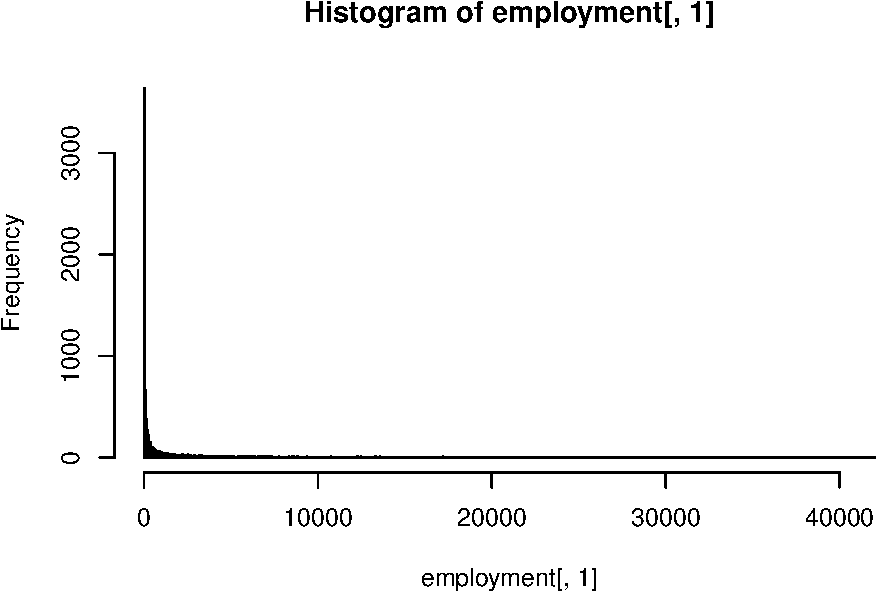
\includegraphics{rampdist_files/figure-latex/unnamed-chunk-3-1.pdf}

or for a closeup:

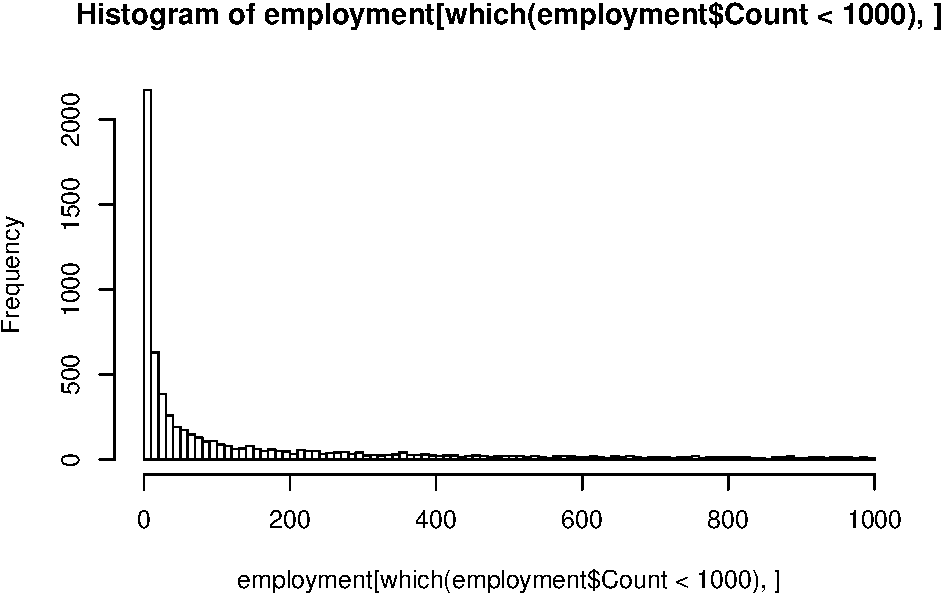
\includegraphics{rampdist_files/figure-latex/unnamed-chunk-4-1.pdf}

but most importantly, it has a \textbf{mean of 3879}, a
\textbf{median of 215}, and \textbf{Q25 of 15}.

\section{Ramp distribution}\label{ramp-distribution}

The most common noise distribution used is a ramp distribution. So what
is a ramp distribution? \[
    p\left( {\delta _{j}}\right) =\left\{ {{
            \begin{array}{ccl} 
            \dfrac{ {1+ b - \delta } }{\left( {b - a} \right)^2}
                    &,&\;\delta \in \mbox{ }\left[ {1+a,1+b} \right] \\ 
                \dfrac{ {\delta - (1 - b)} }{\left( {b - a} \right)^2} 
                &,&\;\delta \in \left[ {1 - b,1 - a} \right] \\ 
                0&,&\;\mbox{ otherwise } \\
                 \end{array}
        }}\right. 
\] with a cumulative distribution of \[
        F\left( {\delta _{j}}\right) =\left\{ {{
                \begin{array}{*{20}c}
                {\mbox{0},\;\delta < {2-b} } \\ 
                {{\left[ {\left( {\delta - (1-b)} \right)^2} \right]} 
                  {\left/ {\vphantom {{\left[ {\left( {\delta - (1-b)} \right)^2} \right]} 
                  {\left[ {2\left( {b - a} \right)^2} \right]}}} \right. } {\left[ {2\left( {b - a} \right)^2} \right]},\;\delta \in \left[ {1 - b,1 - a} \right]\mbox{ }} \\
                  {\mbox{0.5}, \;\delta \in \mbox{ }\left( {1-a,1+a} \right)\mbox{ }} \\
                  {\mbox{0.5} + {\left[ {\left( {b - a} \right)^2 - \left( {1+b - \delta } \right)^2} \right]}
                  {\left/ {\vphantom {{\left[ {\left( {b - a} \right)^2 - \left( {1+b - \delta } \right)^2} \right]}
                  {\left[ {2\left( {b - a} \right)^2} \right]}}} \right. } {\left[ {2\left( {b - a} \right)^2} \right]},\;\delta \in \mbox{ }\left[ {1+a,1+b} \right]\mbox{ 
                    }} \\ 
                    {\mbox{1}, \;\delta > {1+b} } \\ \end{array}}}\right. 
\]

\begin{Shaded}
\begin{Highlighting}[]
\NormalTok{dramp <-}\StringTok{ }\NormalTok{function(x,a,b) \{}
  \NormalTok{if ( b<}\StringTok{ }\NormalTok{a) \{}
    \NormalTok{c <-}\StringTok{ }\NormalTok{a}
    \NormalTok{a <-}\StringTok{ }\NormalTok{b}
    \NormalTok{b <-}\StringTok{ }\NormalTok{c}
  \NormalTok{\}}
  \NormalTok{part1 <-}\StringTok{ }\KeywordTok{which}\NormalTok{(x <}\StringTok{ }\DecValTok{1}\NormalTok{-}\StringTok{ }\NormalTok{b )}
  \NormalTok{part2 <-}\StringTok{ }\KeywordTok{intersect}\NormalTok{(}\KeywordTok{which} \NormalTok{(x >=}\StringTok{ }\DecValTok{1}\NormalTok{-b),}\KeywordTok{which}\NormalTok{(x <=}\StringTok{ }\DecValTok{1}\NormalTok{-a))}
  \NormalTok{part3 <-}\StringTok{ }\KeywordTok{intersect}\NormalTok{(}\KeywordTok{which} \NormalTok{(x >}\StringTok{ }\DecValTok{1}\NormalTok{-a), }\KeywordTok{which}\NormalTok{(x<}\StringTok{ }\DecValTok{1}\NormalTok{+a))}
  \NormalTok{part4 <-}\StringTok{ }\KeywordTok{intersect}\NormalTok{(}\KeywordTok{which} \NormalTok{(x >=}\StringTok{ }\DecValTok{1}\NormalTok{+a),}\KeywordTok{which}\NormalTok{(x <=}\StringTok{ }\DecValTok{1}\NormalTok{+b))}
  \NormalTok{part5 <-}\StringTok{ }\KeywordTok{which}\NormalTok{(x >}\StringTok{ }\DecValTok{1}\NormalTok{+}\StringTok{ }\NormalTok{b )}

  \NormalTok{y <-}\StringTok{ }\NormalTok{x}
  \NormalTok{y[part1] <-}\StringTok{ }\DecValTok{0}
  \NormalTok{y[part2] <-}\StringTok{ }\NormalTok{(x[part2] -}\StringTok{ }\NormalTok{(}\DecValTok{1}\NormalTok{-b))/}\StringTok{ }\NormalTok{( b -}\StringTok{ }\NormalTok{a )^}\DecValTok{2}
  \NormalTok{y[part3] <-}\StringTok{ }\DecValTok{0}
  \NormalTok{y[part4] <-}\StringTok{ }\NormalTok{( }\DecValTok{1} \NormalTok{+}\StringTok{ }\NormalTok{b -x[part4])/}\StringTok{ }\NormalTok{( b -}\StringTok{ }\NormalTok{a )^}\DecValTok{2}
  \NormalTok{y[part5] <-}\StringTok{ }\DecValTok{0}
  \KeywordTok{return}\NormalTok{(y)}
\NormalTok{\}}

\NormalTok{invcramp <-}\StringTok{ }\NormalTok{function(y,a,b) \{}
  \NormalTok{part1 <-}\StringTok{ }\KeywordTok{intersect}\NormalTok{(}\KeywordTok{which}\NormalTok{(y>}\FloatTok{0.5}\NormalTok{),}\KeywordTok{which}\NormalTok{(y<=}\DecValTok{1}\NormalTok{))}
  \NormalTok{part2 <-}\StringTok{ }\KeywordTok{intersect}\NormalTok{(}\KeywordTok{which}\NormalTok{(y<=}\FloatTok{0.5}\NormalTok{),}\KeywordTok{which}\NormalTok{(y>=}\DecValTok{0}\NormalTok{))}
  \NormalTok{part3 <-}\StringTok{ }\KeywordTok{intersect}\NormalTok{(}\KeywordTok{which}\NormalTok{(y<}\DecValTok{0}\NormalTok{),}\KeywordTok{which}\NormalTok{(y>}\DecValTok{1}\NormalTok{))}
  \NormalTok{x <-}\StringTok{ }\NormalTok{y}
  \NormalTok{x[part1] <-}\StringTok{  }\DecValTok{1}\NormalTok{+b -}\StringTok{ }\NormalTok{((}\DecValTok{1-2}\NormalTok{*(y[part1]-}\FloatTok{0.5}\NormalTok{))*(b-a)^}\DecValTok{2}\NormalTok{)^}\FloatTok{0.5}
  \NormalTok{x[part2] <-}\StringTok{  }\DecValTok{1}\NormalTok{-b +}\StringTok{ }\NormalTok{((  }\DecValTok{2}\NormalTok{*(y[part2]    ))*(b-a)^}\DecValTok{2}\NormalTok{)^}\FloatTok{0.5}
  \NormalTok{x[part3] <-}\StringTok{  }\DecValTok{0}
  \KeywordTok{return}\NormalTok{(x)}
  \NormalTok{\}}
\end{Highlighting}
\end{Shaded}

\noindent where \(a={c}/{100}\) and \(b={d}/{100}\) are constants chosen
such that the true value is distorted by a minimum of \(c\) percent and
a maximum of \(d\) percent. This produces a random noise factor centered
around 1 with distortion of at least \(c\) and at most \(d\) percent.

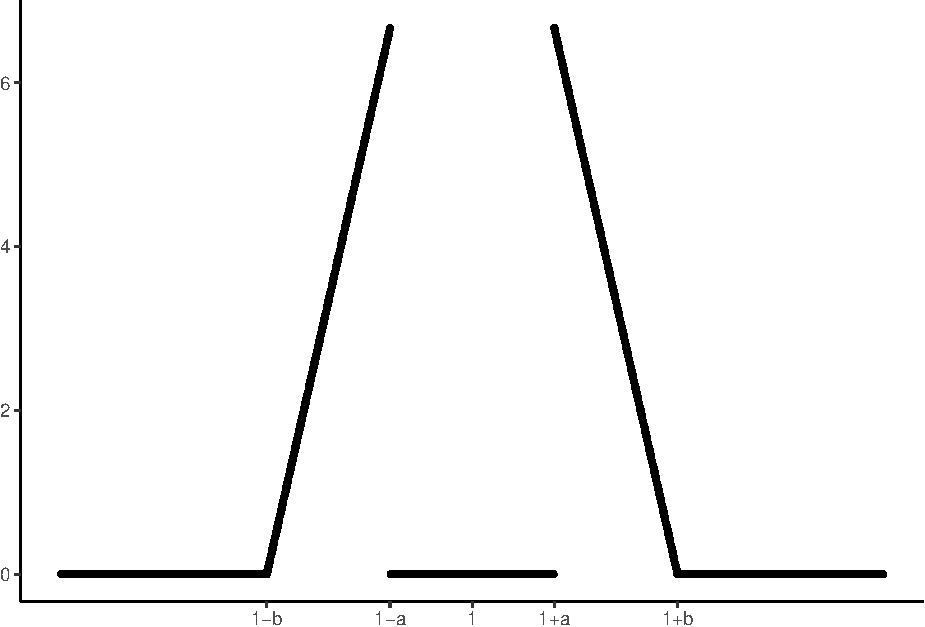
\includegraphics{rampdist_files/figure-latex/plot_ramp-1.pdf}
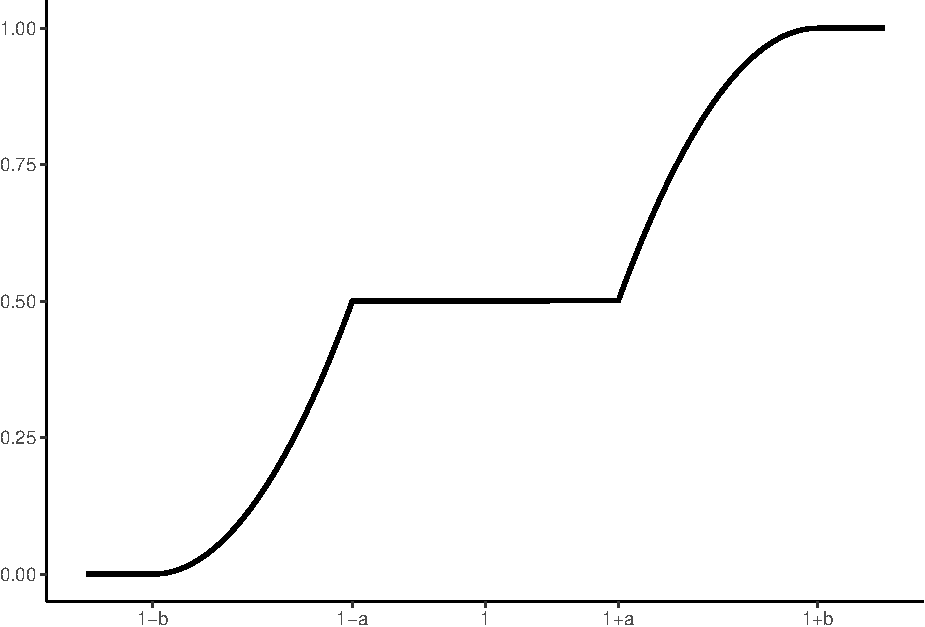
\includegraphics{rampdist_files/figure-latex/plot_cum_ramp-1.pdf}

\section{Distorting the data}\label{distorting-the-data}

Applying the multiplicative noise to the counts yields protected counts.
Since the mean of the noise distribution is unity by design, the two
distributions are likely to have similar means.

\begin{Shaded}
\begin{Highlighting}[]
\NormalTok{employment$uniform <-}\StringTok{ }\KeywordTok{runif}\NormalTok{(}\KeywordTok{nrow}\NormalTok{(employment))}
\NormalTok{employment$fuzzfactor <-}\StringTok{ }\KeywordTok{invcramp}\NormalTok{(employment$uniform,}\FloatTok{0.1}\NormalTok{,}\FloatTok{0.25}\NormalTok{)}
\NormalTok{employment$NoisyCount <-}\StringTok{ }\KeywordTok{round}\NormalTok{(employment$Count *}\StringTok{ }\NormalTok{employment$fuzzfactor,}\DecValTok{0}\NormalTok{)}
\end{Highlighting}
\end{Shaded}

If we compare the original data

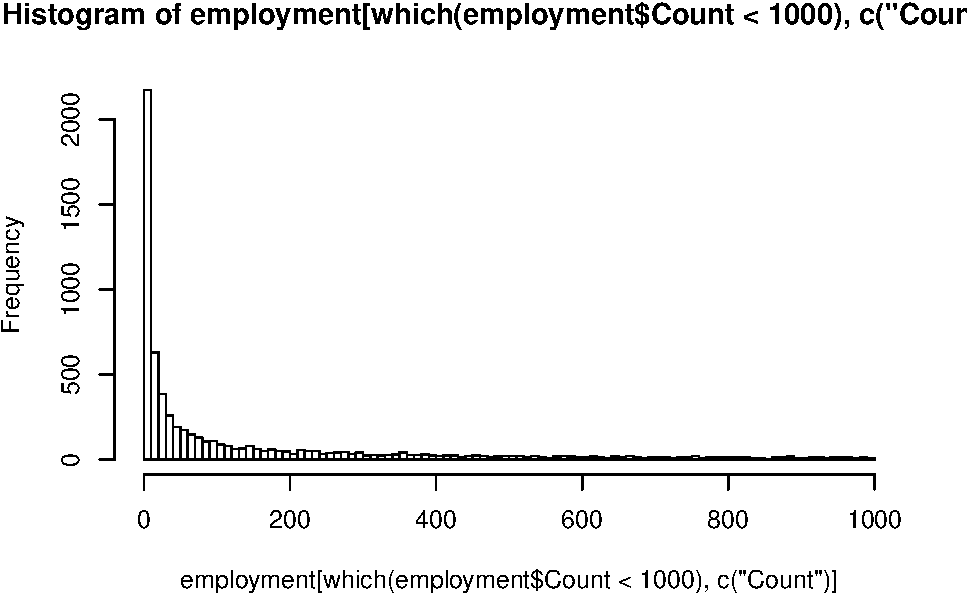
\includegraphics{rampdist_files/figure-latex/unnamed-chunk-6-1.pdf}

against the protected data

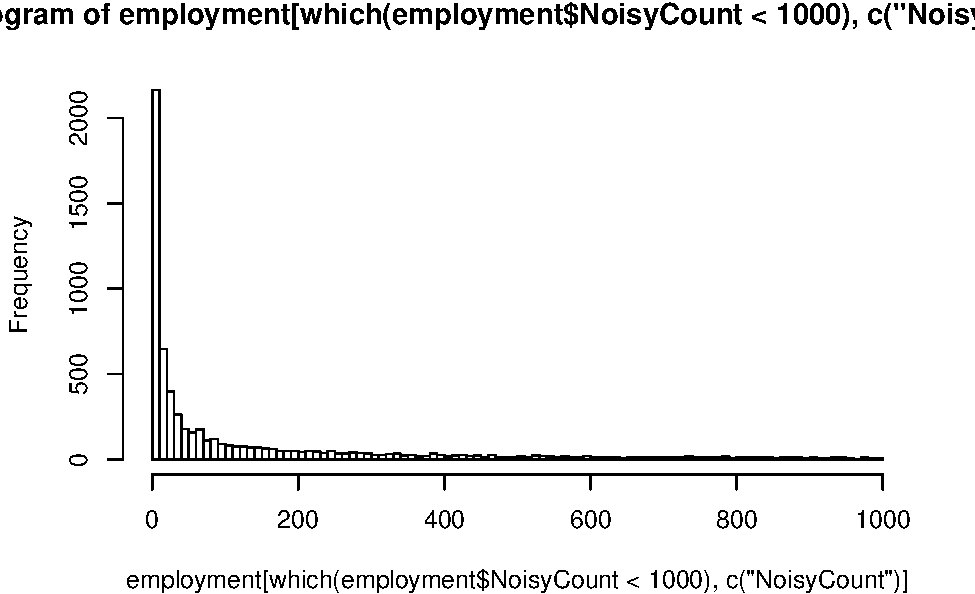
\includegraphics{rampdist_files/figure-latex/unnamed-chunk-7-1.pdf}

we see very similar distributions. The user can verify that the
univariate statistics are very similar: the raw data has a mean of
3878.9 against a mean of 3860.2 in the protected data.


\end{document}
